\section{Operational Amplifiers}\label{sec:Op-Amps}
\begin{definition}[Op-Amp]\label{def:Op-Amp}
  An \emph{op-amp}, (\emph{operational amplifier}), is a active circuit element that is a 2-port network element.
  An circuit symbol for an op-amp is shown in \Cref{fig:Op-Amp}.
\end{definition}

\begin{figure}[h!tbp]
  \centering
  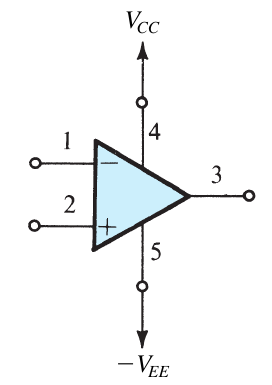
\includegraphics[scale=0.85]{./Op-Amp.png}
  \caption{Complete Circuit Symbol for an Op-Amp \parencite[p.~60]{sedraTextbook7}}
  \label{fig:Op-Amp}
\end{figure}

Typically, terminals 4 and 5 are \textbf{not} included in circuit schematics, as they are implied to exist, because the \nameref{def:Op-Amp} requires input power to operate.

\begin{definition}[Open-Loop Gain]\label{def:Open-Loop_Gain}
  The \emph{open-loop gain} of an \nameref{def:Op-Amp}, typically represented with \OpenLoopGain{} is the gain in voltage at the output given an input voltage.
  The equation for the open-loop gain is given in \Cref{eq:Open-Loop_Gain}.

  \begin{equation}\label{eq:Open-Loop_Gain}
    \OpenLoopGain = \frac{V_{O}}{V_{+} - V_{-}}
  \end{equation}
\end{definition}

\subsection{The Ideal Op-Amp}\label{subsec:Ideal_Op-Amp}
The ideal \nameref{def:Op-Amp} is one that has:
\begin{enumerate}[noitemsep]
\item Infinite input impedance
\item Zero output impedance
\item Zero common-mode gain/infinite common-mode rejection
\item Infinite \nameref{def:Open-Loop_Gain}
\item Infinite bandwidth (There is no distortion of the output signal due to amplification.)
\end{enumerate}

This can be summarized using just two equations, shown in \Cref{eq:Ideal_Op-Amp-Voltage,eq:Ideal_Op-Amp-Current}.
\begin{subequations}
  \begin{equation}\label{eq:Ideal_Op-Amp-Voltage}
    V_{+} = V_{-}
  \end{equation}
  \begin{equation}\label{eq:Ideal_Op-Amp-Current}
    I_{+} = I_{-} = 0
  \end{equation}
\end{subequations}

When connecting an \nameref{def:Op-Amp}, even an ideal one, to a circuit, the \nameref{def:Closed-Loop_Gain} becomes a factor.

\begin{definition}[Closed-Loop Gain]\label{def:Closed-Loop_Gain}
  The \emph{closed-loop gain} occurs when an \nameref{def:Op-Amp} is connected to a surrounding circuit.
  It's defining equation is shown in \Cref{eq:Closed-Loop_Gain}.

  \begin{equation}\label{eq:Closed-Loop_Gain}
    \ClosedLoopGain = \frac{V_{O}}{V_{I}}
  \end{equation}
\end{definition}


%%% Local Variables:
%%% mode: latex
%%% TeX-master: "../ECE_311-Engineering_Electronics-Reference_Sheet"
%%% End:
